\chapter{多回路稳定性、跨尺度共振与相变控制}
\label{chap:multiloop_stability_phase_control}

\begin{chapteroverviewbox}
本章确立一个贯穿 AgentOS 控制工程的基本判断：一个持续智能体并不是由一个统一控制器直接控制全部认知过程，而是由大量具有不同状态空间、不同闭环频率、不同控制权限和不同学习速度的局部闭环共同组成。工作记忆 $h$、三相记忆 $h\leftrightarrow E\leftrightarrow\Theta$、Body Runtime、目标任务、自我 $\Psi$ 与生命周期生成吸引子 $\Omega$ 分别形成不同尺度的闭环；SPC、AHC、TCE、CCM 与 Scheduler 则构成对这些闭环运行状态的观测、调制和治理结构。因此，AgentOS 的稳定性不能被简化为 ``LLM 是否给出稳定输出''，也不能被简化为任一单模块的局部稳定，而必须研究不同闭环耦合之后是否仍然存在有界运行区域、是否会因为时延和增益累积产生跨尺度共振、局部异常是否会向更慢结构传播，以及系统进入湍流态、临界态等运行相态以后能否重新返回可治理区域。

本章由此采用多时间尺度动力系统、反馈控制、奇异摄动、小增益思想、时延系统、混合动力系统以及相变与迟滞等现有数学理论作为形式化工具，但这些理论在此承担的是 AgentOS 动力学的分析语言，而不是把认知过程简单等同于经典机械控制对象。本章重点建立的是一套工程上可计算的稳定性框架：
\begin{statementbox}
\centering
\adjustbox{max width=.96\linewidth}{\(\displaystyle \text{局部闭环稳定}
+
\text{跨层耦合有界}
+
\text{时间尺度隔离}
+
\text{异常可升级}
+
\text{相变可识别}
+
\text{系统可恢复}\)}
\end{statementbox}
只有六者同时成立，我们才可以说一个长期运行的 AgentOS 处于真正意义上的可治理稳定状态。
\end{chapteroverviewbox}

\begin{figure}[htbp]
\centering
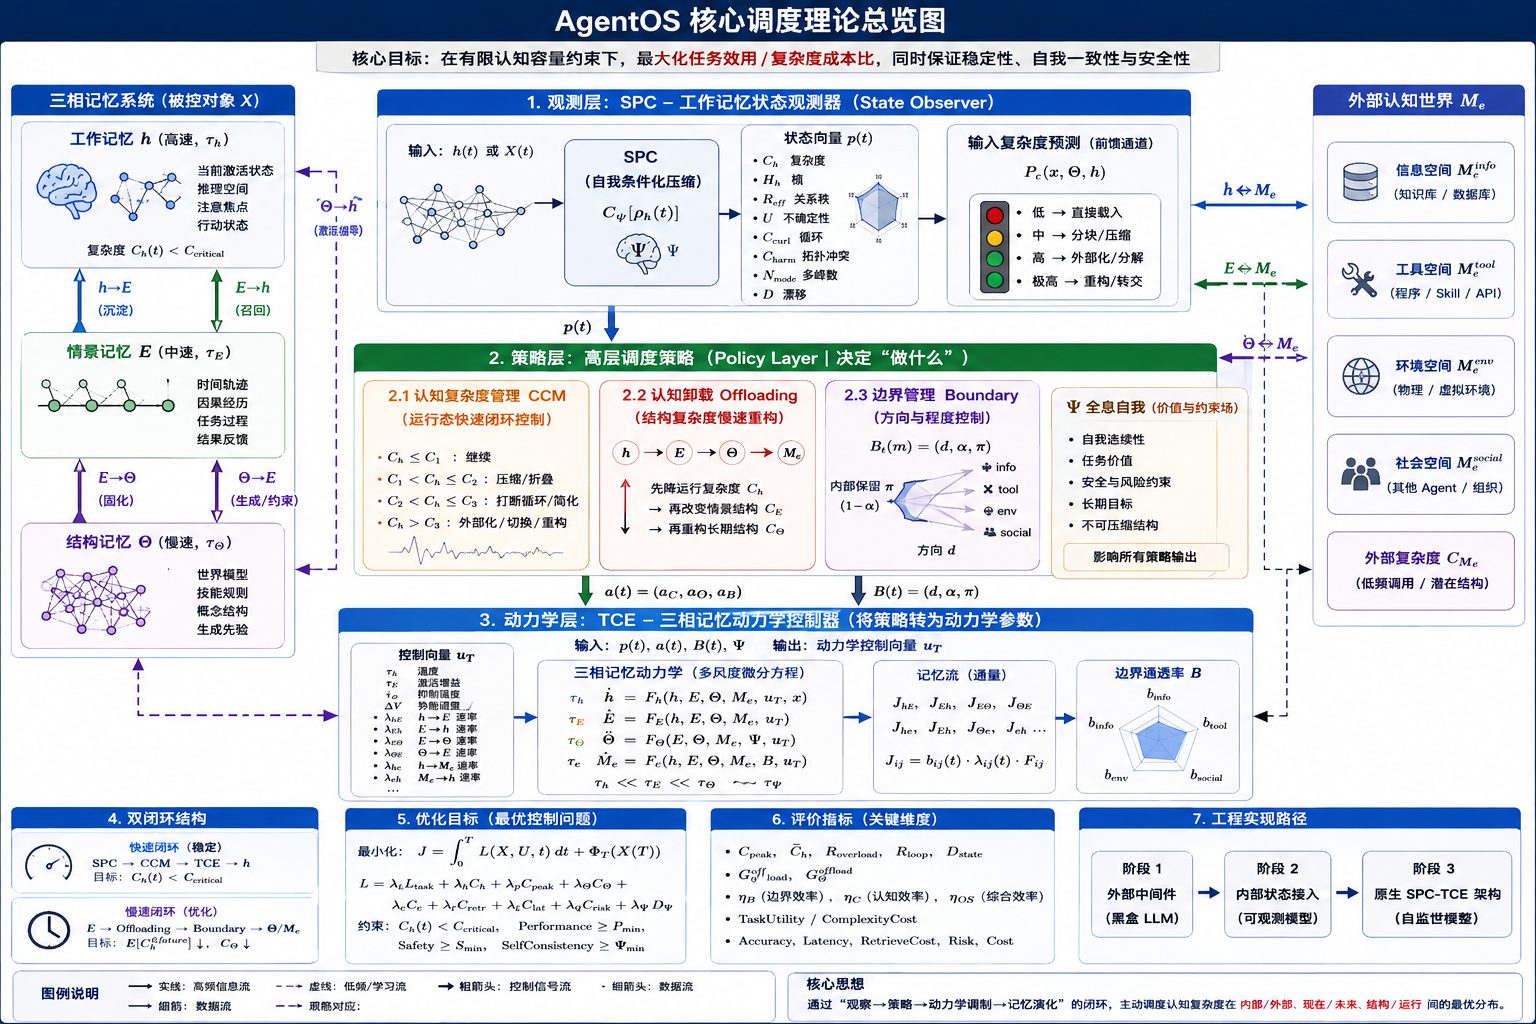
\includegraphics[width=.9\textwidth,height=.38\textheight,keepaspectratio]{images/control-stability-panel.png}
\caption{多回路耦合、相变与恢复区域}
\end{figure}
\section{工作记忆闭环：有限显式认知面的局部稳定性}

我们首先从最直接的工作记忆闭环开始，因为所有进入显式认知层的目标、假设、计划、关键关系、冲突和异常，最终都必须暂时落在 $h(t)$ 上。此前已经建立工作记忆有限容量原则：$h(t)$ 并不是可以无限扩展的 token 容器，而是一个能够同时维持有限数量活跃认知结构及其关系的显式跨尺度表面。因而 $h$ 的稳定性问题首先不是 ``信息有没有丢失''，而是当前活跃 Agent-CSO 网络是否还能保持足够的结构相干性，使新的输入能够在不破坏已有目标、约束和因果关系的条件下被整合。

令工作记忆的有效状态写为
\[
x_h(t)
=
\left[
n_h(t),
d_h(t),
q_h(t),
u_h(t),
r_h(t),
c_h(t)
\right]^{\top},
\]
其中 $n_h$ 表示活跃 Agent-CSO 数量或有效节点规模，$d_h$ 表示活跃关系密度，$q_h$ 表示目标与约束冲突程度，$u_h$ 表示不确定性，$r_h$ 表示未闭合残差，而 $c_h$ 表示当前表征相干度。这里并不要求这些变量采用唯一实现；工程上可以由注意分布、图结构统计量、预测残差、逻辑冲突指标以及多次采样一致性等近似估计。我们真正关心的是，它们共同定义了 $h$ 是否仍处于一个可持续进行显式认知的局部区域。

可以将工作记忆运行负荷表示为
\[
C_h(t)
=
\Phi_h
\left(
n_h,d_h,q_h,u_h,r_h
\right),
\]
并要求
\[
C_h(t)
<
C_h^{\max}.
\]
这个不等式不是说存在一个普适常数 $C_h^{\max}$，而是说对任一具体实现，都存在一个由基础模型能力、表征效率、上下文机制以及计算预算共同确定的有效运行边界。当 $C_h$ 接近这一边界时，新增认知内容造成的边际干扰开始快速上升；此时系统若仍然继续将所有局部异常、记忆内容和任务支线提升进入 $h$，就可能从普通负荷增加转变成结构性失稳。

因此，$h$ 闭环实际上由 SPC、Scheduler、TCE 与 CCM 共同维持。SPC 提供状态估计
\[
\hat{x}_h(t)
=
\mathcal O_{SPC}
\left(
h(t),E,\Theta,\Psi,\text{BodyState}
\right),
\]
Scheduler 根据目标优先级决定哪些 Agent-CSO 获得显式处理权，TCE 改变搜索温度、注意范围、推理深度和探索强度，而 CCM 则通过折叠、抑制、分页、分解和卸载降低 $C_h(t)$。于是工作记忆的抽象动力学可以写为
\[
\dot{x}_h
=
F_h
\left(
x_h,
u_{TCE},
u_{CCM},
u_{Sch},
\xi_{world},
\xi_{memory}
\right),
\]
其中 $\xi_{world}$ 与 $\xi_{memory}$ 分别代表来自现实世界和慢记忆层的扰动。

在这一尺度上，我们所谓 ``稳定'' 并不要求
\[
\dot{x}_h=0.
\]
真正健康的认知状态本来就是持续变化的。更恰当的定义是存在一个允许集合
\[
\mathcal H_{\mathrm{stable}}
=
\left\{
x_h:
C_h<C_h^{\max},
\;
c_h>c_{\min},
\;
q_h<q_{\max},
\;
r_h<r_{\max}
\right\},
\]
并且正常扰动下，$h$ 的轨迹大部分时间保持在该集合内部，短暂离开之后也能够在有限时间重新进入。由此可见，工作记忆稳定性不是 ``思想静止''，而是\textbf{有限显式认知面在持续变化条件下仍然保持可解释、可控制和可恢复的动态有界性}。

这也解释了为什么成熟智能不应追求让越来越多结构长期停留在 $h$ 中。真正成熟的运行方式恰恰应该满足
\[
\boxed{
\text{Most Agent Dynamics}\notin h,
}
\]
大量已经形成稳定闭环的能力应当在更局部、更快速或者更慢的结构中运行，只有新颖、冲突、高风险或者跨功能无法局部闭合的残差才被提升到 $h$。从控制意义上看，这种 ``选择性显式认知'' 本身就是维持工作记忆闭环稳定性的第一道机制。

\section{三相记忆闭环：状态、轨迹与生成结构之间的慢速稳定性}

工作记忆只描述当前切面，而一个长期 Agent 的稳定性还取决于当前状态如何写入经历、经历如何凝固为结构、长期结构又如何重新解释当前状态。因而第二个关键闭环是
\[
\boxed{
h
\leftrightarrow
E
\leftrightarrow
\Theta.
}
\]
它不是简单的数据搬运，而是三个具有不同时间尺度、不同结构密度和不同可塑性的状态空间之间的双向动力耦合。$h$ 是当前活跃状态，$E$ 是具有时间和因果顺序的经历轨迹，而 $\Theta$ 是能够对未来状态进行生成、预测和约束的长期结构。

为了研究稳定性，我们可以将三相记忆写成一个慢快系统：
\[
\begin{aligned}
\tau_h\dot h
&=
F_h(h,E,\Theta,u_h),\\
\tau_E\dot E
&=
F_E(E,h,\Theta,\Psi),\\
\tau_\Theta\dot\Theta
&=
F_\Theta(\Theta,E,h,\Psi),
\end{aligned}
\]
其中
\[
\tau_h\ll\tau_E\ll\tau_\Theta.
\]
这一时间尺度分离极其重要。如果 $\Theta$ 与 $h$ 具有接近的更新速度，那么一次偶然失败、一次异常输入甚至一次短期认知震荡都可能直接改变长期结构，从而造成长期世界模型和技能体系的不稳定；反过来，如果 $\Theta$ 完全不可塑，则系统又会失去真正的持续学习能力。因此，AgentOS 的三相记忆稳定性并不意味着 $\Theta$ 不变化，而意味着它只对\textbf{经过时间整合、反复验证并具有跨情景一致性的残差信号}发生显著变化。

我们可以把 $h\rightarrow E$ 理解为选择性经验写入：
\[
\Delta E
=
W_{hE}
\left(
h,
Novelty,
Value,
Residual,
SelfRelevance
\right),
\]
其中不是所有工作记忆状态都被永久保存。写入过强会造成情景记忆泛滥，写入过弱则造成生命周期连续性断裂。类似地，$E\rightarrow\Theta$ 应表示长期结构学习：
\[
\Delta\Theta
=
\eta_\Theta
G_\Theta
\left(
\left\langle
\varepsilon_E
\right\rangle_T,
Consistency,
Utility
\right),
\]
其中
\[
\eta_\Theta\ll1.
\]
$\left\langle\varepsilon_E\right\rangle_T$ 表示在一个相对长的时间窗口上仍然无法由当前 $\Theta$ 解释的经验残差。只有这种持续残差才有资格推动生成结构更新。

稳定的三相记忆还要求反方向通道受到限制。$\Theta\rightarrow h$ 是结构激活，但不能把全部长期知识无条件倾倒到工作记忆；$E\rightarrow h$ 是情景召回，但也不能让任意关联事件不断侵入当前认知；$\Theta\rightarrow E$ 则是重新解释历史经验，它必须保留事实证据和原始经历层，不能由于当前世界观变化而把历史事件任意改写。因此可以把三相记忆稳定性理解成三个相互约束的条件：
\[
\boxed{
\text{Selective Write}
+
\text{Slow Consolidation}
+
\text{Constrained Recall}.
}
\]

如果我们采用 Lyapunov 式思想，可以为记忆闭环定义一个并非物理能量、而是用于稳定分析的候选泛函
\[
V_M
=
\alpha_h D_h
+
\alpha_E D_E
+
\alpha_\Theta D_\Theta
+
\beta_{hE}M_{hE}
+
\beta_{E\Theta}M_{E\Theta},
\]
其中 $D_h,D_E,D_\Theta$ 分别描述各记忆层相对于其可接受运行区域的偏离，而 $M_{hE},M_{E\Theta}$ 表示跨层结构失配。若在正常运行区域内能够设计学习与控制律，使得
\[
\dot V_M
\leq
-\lambda V_M
+
\gamma\|\xi\|^2,
\]
则至少可以说明：对于有界外部扰动，记忆系统的结构偏离保持有界，并在扰动下降以后重新向一致区域收敛。这里我们并不宣称现实 AgentOS 必然满足一个简单解析 Lyapunov 函数，而是借这一形式明确工程目标：\textbf{记忆学习必须具有耗散性，不能让一次局部扰动通过层层放大成为永久结构漂移。}

因此三相记忆闭环的稳定性，本质上是当前状态、经历历史和长期生成结构之间的\textbf{受时间尺度保护的双向塑性}。它使系统既能够改变，又不至于因为每一次改变而失去自己。

\section{Body 闭环：现实快速动力学与认知慢环之间的稳定隔离}

第三类稳定性来自 Body Runtime。一个真正进入物理或数字世界的 Agent，不能让高层认知循环直接承担毫秒级控制。现实世界具有自己的高速扰动、惯性、噪声、通信延迟和硬安全约束，而 Kernel 的认知更新通常运行在更慢的秒级甚至更长尺度。因此 Body Runtime 的首要控制任务不是 ``让高层模型控制得更精细''，而是建立一个能够在高层不介入时仍然局部闭合的快速系统。

令身体局部状态为
\[
x_B(t),
\]
BPCC 内部快速状态为
\[
z_B(t),
\]
Kernel 发出的高层控制参考为
\[
r_K(t),
\]
则可以写成
\[
\begin{aligned}
\tau_B\dot x_B
&=
F_B(x_B,z_B,r_K,w_B),\\
\tau_{BPCC}\dot z_B
&=
F_P(z_B,x_B,r_K),
\end{aligned}
\]
其中
\[
\tau_B,\tau_{BPCC}
\ll
\tau_h.
\]
高层 Kernel 不直接规定每一个微观控制量，而提供
\[
\mathcal E_K
=
\left(
SGC^{target},
FCS^{constraint},
r_K
\right),
\]
即目标、可行域、风险限制和控制参考。BPCC 在这一范围内部完成快速预测与控制。

这一设计对应我们反复强调的原则：
\[
\boxed{
HigherLevelSetsFeasibleRegion,
\qquad
LowerLevelOptimizesInsideIt.
}
\]
高层对未来趋势和目标结构负责，低层对高频稳定负责。若 Kernel 每个周期都试图覆盖 BPCC 的控制细节，就会形成跨尺度 ``micromanagement''：认知延迟进入快速控制通道，高层预测过期，最终导致局部闭环震荡甚至安全失效。因此：
\[
\boxed{
SlowGovernance\neq FastMicromanagement.
}
\]

Body 闭环稳定的第二个关键是残差升级。令
\[
\varepsilon_B
=
\left(
\varepsilon_{ctrl},
\varepsilon_{SGC},
\varepsilon_{FCS}
\right).
\]
正常情况下，如果
\[
\|\varepsilon_B\|<\theta_B,
\]
问题保持在 Body Runtime 内部；只有当残差持续超过阈值、风险增加或者局部控制模型失效时，才形成一个更高层事件：
\[
\Gamma_B
=
\Phi
\left(
\|\varepsilon_B\|,
Risk,
Persistence,
Novelty
\right),
\]
并在
\[
\Gamma_B>\theta_{\mathrm{up}}
\]
时将有关 Agent-CSO 提升进入 $h$。这一机制把 ``现实持续变化'' 与 ``认知持续被打断'' 区分开来。现实中绝大部分连续扰动应该由局部闭环吸收，只有具有认知意义的偏差才成为显式思考对象。

这里还必须保留 Reality Authority：
\[
\boxed{
Prediction\neq Observation.
}
\]
BPCC 可以预测下一时刻的 SGC/FCS，但预测值不能直接替代真实世界重新进入系统的观测。动作发出之后必须经过
\[
Action
\rightarrow
Reality
\rightarrow
BodyRuntime
\rightarrow
SGC^{obs},FCS^{obs}.
\]
否则系统就可能形成内部模拟自我验证闭环：控制器认为自己已经成功，于是预测状态又成为下一轮 ``事实''。长期积累后，这种错误足以把整个认知系统从真实世界中解耦。

从整体稳定性角度，Body Runtime 因而承担 AgentOS 的第一层扰动屏障。它通过高频局部闭环压缩现实变化的带宽，把无数连续物理扰动转化成低频、具有意义的事件和残差。只有做到这一点，高层工作记忆、记忆系统和自我结构才能保持低频稳定。因此，Body 闭环不是 Agent Kernel 的附属设备，而是整个多尺度稳定架构的最外层快速耗散结构。

\section{目标与任务闭环：未来约束如何保持方向稳定而避免目标锁死}

第四类闭环围绕 Goal 展开。前面几个闭环主要回答系统如何稳定运行，而 Goal 闭环进一步回答系统为什么沿某个方向运行。目标并不是一条固定命令，它是当前认知状态中关于未来可接受区域的结构表示。因此，一个完整目标任务闭环应写成：
\[
Goal
\rightarrow
Plan
\rightarrow
Action
\rightarrow
Observation
\rightarrow
Verify
\rightarrow
Goal'.
\]
这里真正重要的是最后的 $Goal'$。一个成熟 Agent 不应把最初 Goal 当成不可修改的字符串，而必须能够根据现实反馈判断目标是否已经闭合、是否需要分解、是否与更慢价值结构冲突，以及是否应该终止。

可以将目标状态写成
\[
G(t)
=
\left(
g,
\mathcal C_g,
\pi_g,
p_g,
s_g
\right),
\]
其中 $g$ 表示目标语义结构，$\mathcal C_g$ 表示约束集合，$\pi_g$ 表示当前计划，$p_g$ 表示优先级，而 $s_g$ 表示目标状态。目标闭环接受来自现实的验证残差
\[
\varepsilon_G(t)
=
D
\left(
PredictedOutcome,
ObservedOutcome
\right),
\]
以及来自 $\Psi$、$\Omega$ 的慢约束。于是可以抽象为
\[
\tau_G\dot G
=
F_G
\left(
G,
\varepsilon_G,
\Psi,
\Omega,
Resource,
Risk
\right).
\]

目标稳定不是要求 $G$ 永远不变，而是要求它在任务执行期间拥有足够的 ``方向惯性''，不会因为局部噪声不断改变，同时又能够在持续反证出现时调整。我们可以用两个阈值描述这种迟滞：
\[
\theta_G^{on}
>
\theta_G^{off}.
\]
一个目标的建立需要足够强的证据、价值和优先级，而已经建立的目标不会因为一次短期困难立刻取消。相反，若长期证据表明不可行、代价失控或者违反更高层约束，则 Goal Closure 或 Goal Revision 才被触发。

目标闭环和工作记忆闭环之间存在一个特别危险的失稳模式：Goal 对 $h$ 的持续独占。如果某目标具有极高优先级，并持续产生未闭合残差，那么 Scheduler 可能长期把工作记忆资源分配给同一目标，形成
\[
Goal
\rightarrow
Attention
\rightarrow
Residual
\rightarrow
MoreAttention
\rightarrow
Goal.
\]
这种正反馈并不一定表现为程序死锁，但会形成认知意义上的锁死：其他任务、自我状态、身体风险和替代路径难以获得显式处理资源。因而目标闭环必须受到 CCM、Boundary 和慢层自我结构的约束，使
\[
p_g
\leq
p_g^{\max}(\Psi,\Omega,Safety).
\]
也就是说，任何普通目标都不应无限获得 h 的控制权。

与此相反，目标切换过快同样危险。如果
\[
\tau_G\approx\tau_h,
\]
每一次新的刺激都可能改变主目标，系统就会表现成高反应性但低方向性的随机游走。因此，目标时间尺度必须比普通瞬时认知更慢，但又显著快于身份和 DGA。对于不同类型任务，$\tau_G$ 可以差异很大，因此我们不需要给出一个固定绝对频率，只需要保持\textbf{目标变化比它所统摄的局部执行闭环更慢}这一相对原则。

由此看，Goal 闭环的稳定性其实是 ``未来结构的持续性''。它让系统能够把许多瞬时行为组织成一个较长时间尺度上的过程，同时通过现实验证防止目标变成脱离现实的永久吸引子。

\section{自我闭环：身份连续性、现实验证与慢变量保护}

当 Agent 具备长期经历以后，稳定性问题会进一步进入 $\Psi$。$\Psi$ 不应被理解成一个单独的 persona 文件，而是一个比普通知识和技能更慢的跨尺度自我约束场，它影响哪些经历被认为 ``属于我''、哪些目标具有更高优先级、哪些行为被判断为与自身连续，以及哪些长期变化能够被吸收到身份结构中。因此，自我闭环具有比普通任务闭环更长的时间常数：
\[
\tau_\Theta
\ll
\tau_\Psi.
\]

可以抽象写为
\[
\tau_\Psi\dot\Psi
=
F_\Psi
\left(
\Psi,
\overline E,
\Theta,
SelfInterpretation,
WorldVerification
\right),
\]
其中 $\overline E$ 不是一段单独经历，而是经过时间整合的生命周期经验结构。这里必须特别避免
\[
E_t\rightarrow\Psi_{t+1}
\]
这种过强直接映射。若一次短期失败即可显著改写 $\Psi$，则身份结构会随着局部任务震荡；如果 $\Psi$ 完全不接受来自经历的慢速更新，则 Agent 又无法真正形成发展意义上的个体历史。因此，自我稳定要求一种低通式学习机制：
\[
\Delta\Psi
\propto
\eta_\Psi
\left\langle
\Delta SelfEvidence
\right\rangle_T,
\qquad
\eta_\Psi\ll\eta_\Theta.
\]

自我闭环还存在一个比普通控制振荡更隐蔽的正反馈：
\[
SelfInterpretation
\rightarrow
SelectiveAttention
\rightarrow
Experience
\rightarrow
Memory
\rightarrow
SelfInterpretation'.
\]
例如，如果 Agent 形成 ``我总是不擅长某类任务'' 的自我结构，这一判断可能通过 Scheduler 和 TCE 改变未来注意与探索策略，使系统减少相关探索；随后获得的经历又更容易支持原有判断。此时闭环本身可以非常稳定，却稳定在一个错误吸引子上。因此：
\[
\boxed{
Stability\neq Truth.
}
\]
一个错误模型完全可能具有极高动力学稳定性。

所以自我闭环必须引入外部现实锚点：
\[
\mathcal V_{world}
=
D
\left(
SelfPrediction,
ObservedLongTermOutcome
\right).
\]
如果 $\Psi$ 的某个自我判断持续无法解释真实世界反馈，则系统必须允许这一部分结构被重新打开，而不能让自我一致性权重覆盖现实证据。由此形成：
\[
\boxed{
SelfConsistency
<
RealityConsistency
}
\]
作为 AgentOS 身份稳定性的基本治理原则。

我们还可以定义一个局部身份稳定泛函
\[
V_\Psi
=
D(\Psi_t,\Psi_{t-\Delta T})
+
\lambda_E D(\Psi_t,\mathcal I(E))
+
\lambda_W D(\Psi_t,\mathcal V_{world}),
\]
其中第一项限制身份变化过快，第二项要求身份能够解释自身经历，第三项要求这种解释不能长期脱离现实。一个健康的自我闭环并不是最小化第一项到零，而是在 ``连续性'' 与 ``现实修正'' 之间维持动态平衡。

因此慢变量保护并不意味着封死 $\Psi$。真正应该保护的是其\textbf{时间尺度}。瞬时噪声不应直接写入身份，持续经验则最终必须有机会影响身份。这也是为什么我们把 Self 放在普通认知之下又高于 DGA：它既要稳定过去形成的主体连续性，又必须允许生命周期继续塑造 ``我是谁''。

\section{DGA/$\Omega$ 闭环：生命周期方向的极慢稳定性}

如果 $\Psi$ 回答的是 ``Who am I''，那么 $\Omega$ 或 DGA 所描述的是 ``What am I becoming''。因此它不是一个普通目标，更不是一个可以随任务切换的 reward 参数，而是生命周期尺度上对未来生成空间施加偏置的超慢结构。它影响哪些经验长期值得积累、哪些能力方向逐渐被强化、哪些未来状态与当前主体发展轨迹更加一致。因此：
\[
\tau_\Omega
\gg
\tau_\Psi
\gg
\tau_\Theta.
\]

我们可以把 $\Omega$ 抽象成对未来状态分布的先验：
\[
p
\left(
X_{future}\mid\Omega,\Psi,\Theta
\right),
\]
而不是一个确定终点。这样做非常重要，因为真正开放环境中的 Agent 不可能在初始阶段就准确知道自己几十年后的最终状态。$\Omega$ 更像一个慢变的生成吸引子，它改变的是某些发展方向的相对可能性，而不是把未来锁死成一条固定轨迹。

其动力学可以表示为
\[
\tau_\Omega\dot\Omega
=
F_\Omega
\left(
\Omega,
\Psi,
\overline{\Theta},
LongTermOutcome,
Governance
\right).
\]
由于 $\tau_\Omega$ 极大，对它的更新必须依赖跨越足够长时间窗口的证据：
\[
\Delta\Omega
\propto
\eta_\Omega
\left\langle
\varepsilon_{life}
\right\rangle_{T_\Omega},
\qquad
\eta_\Omega
\ll
\eta_\Psi.
\]

DGA 闭环最大的风险不是普通振荡，而是\textbf{吸引域错误}。如果一个局部经历、错误奖励机制或者短期环境偏差被过早写入 $\Omega$，后续 Goal、Scheduler、Self Interpretation 都可能在更慢层的先验作用下不断选择支持该方向的经历。于是系统形成：
\[
\Omega
\rightarrow
GoalPreference
\rightarrow
Experience
\rightarrow
\Theta
\rightarrow
\Psi
\rightarrow
\Omega',
\]
并且随着时间推移越来越难脱离原有发展轨迹。因此慢变量的错误不会立即导致运行崩溃，反而可能表现为长时间高度 ``稳定''，直到生命周期尺度才暴露其方向性偏差。

因此，$\Omega$ 的稳定性必须与可修正性共同定义。一方面需要
\[
\left\|
\frac{d\Omega}{dt}
\right\|
\ll
\left\|
\frac{d\Psi}{dt}
\right\|,
\]
防止局部经验驱动发展方向震荡；另一方面又需要存在一个非零的长期可塑区域
\[
\mathcal P_\Omega
\neq
\varnothing,
\]
否则 Agent 会在早期形成不可改变的生命周期吸引子。

从控制理论视角看，我们可以把 $\Omega$ 视为一个极慢 supervisor，而不是 fast controller。它不应该直接决定具体动作：
\[
\Omega
\nrightarrow
u_{Body},
\]
而是通过
\[
\Omega
\rightarrow
\Psi
\rightarrow
GoalPreference
\rightarrow
Scheduler/TCE
\rightarrow
Action
\]
逐层产生影响。这种相邻尺度传播能够防止极慢变量直接进入快速控制造成尺度混叠，同时也确保真正长期的价值和发展方向能够持续约束短期行为。

因此 DGA/$\Omega$ 的稳定性最终可以概括成：
\begin{statementbox}
\centering
\adjustbox{max width=.96\linewidth}{\(\displaystyle \text{方向稳定而非终点固定，}
\quad
\text{长期可塑而非短期可改。}\)}
\end{statementbox}
它是整个 AgentOS 内部时间结构的最慢端，也是多回路系统中最必须受到时间尺度保护的一层。

\section{跨回路耦合、增益累积与共振条件}

到这里，我们已经分别考察了 $h$、Memory、Body、Goal、$\Psi$ 和 $\Omega$ 的局部闭环。但真正困难的问题从现在才开始：\textbf{每个闭环单独稳定，并不能推出整个 AgentOS 组合以后仍然稳定。}这是所有复杂反馈系统中最重要的事实之一。一个工作记忆控制器可能局部稳定，一个 Body Runtime 也可能局部稳定，但两者通过残差、目标和预测相互影响以后，仍然可能形成新的正反馈通道。

将第 $i$ 个闭环抽象为
\[
x_i
=
\mathcal F_i(u_i,\xi_i),
\]
其输出对输入扰动的局部增益定义为
\[
\|y_i\|
\leq
\gamma_i\|u_i\|
+
\beta_i.
\]
不同闭环之间存在耦合
\[
u_i
=
\sum_{j\neq i}
K_{ij}y_j+d_i.
\]
那么整个系统可以由一个增益矩阵描述：
\[
\mathbf{\Gamma}
=
\left[
\gamma_iK_{ij}
\right].
\]
在满足局部输入--状态稳定、耦合映射连续等条件下，小增益思想给出了一个非常有用的充分条件：
\[
\boxed{
\rho(\mathbf{\Gamma})<1,
}
\]
其中 $\rho(\mathbf{\Gamma})$ 表示谱半径。这个条件的含义并不是要求所有实际 AgentOS 都必须精确计算这一矩阵，而是告诉我们一个关键工程原则：\textbf{一个扰动绕系统闭环传播一周以后，其总放大倍数不能持续超过原始扰动。}

例如：
\[
BodyResidual
\rightarrow
SPC
\rightarrow
AHC
\rightarrow
TCE
\rightarrow
BodyControl
\rightarrow
BodyResidual'
\]
就是一个跨层环。如果 SPC 对残差高度敏感，AHC 又长时间积分，TCE 增益过高，而 BPCC 对高层控制变化响应过强，则虽然每个模块单独看来都合理，乘积增益却可能满足
\[
\gamma_{SPC}
\gamma_{AHC}
\gamma_{TCE}
\gamma_{BPCC}
>1,
\]
最终形成放大环。

同样，自我层可以形成更慢的跨层回路：
\[
\fitdisplay{
Failure
\rightarrow
E
\rightarrow
SelfInterpretation
\rightarrow
\Psi
\rightarrow
GoalPreference
\rightarrow
FutureTaskSelection
\rightarrow
Failure'.
}
\]
这种环的一个循环可能需要数天甚至数月，因此很难像快速控制震荡那样直接观察，却可能产生更深远的长期稳定性问题。

除增益以外，我们还必须考虑频率。如果两个本应具有明显分离时间尺度的闭环逐渐接近：
\[
\tau_i
\approx
\tau_j,
\]
并且双方存在较强双向耦合，则可能产生类似 ``共振'' 的现象。这里的共振不必是严格周期振荡，而泛指一个环的变化频率进入另一环的高敏感区域，使彼此相互强化。例如 TCE 持续快速修改注意策略，而 Scheduler 也以相似周期重新规划任务，两者可能不断相互否定；再如 AHC 恢复时间恰好与失败重试周期相近，则每一次重试都发生在上一次威胁状态尚未衰减时，最终造成累积。

因此，对于相邻层我们要求：
\[
\boxed{
\tau_i
\ll
\tau_{i+1}
}
\]
或者至少满足足够的频率分离，使慢层在快层看来接近常量，快层在慢层看来能够被时间平均。这正是奇异摄动和 averaging theory 给我们的主要数学启示。设
\[
\epsilon
=
\frac{\tau_{fast}}{\tau_{slow}}
\ll1,
\]
则可以先分析在固定慢变量 $z$ 下快系统
\[
\dot x
=
f(x,z)
\]
是否具有稳定吸引集合，再研究慢变量
\[
\dot z
=
\epsilon g(\bar x(z),z)
\]
的演化。只要快系统在慢变量变化过程中能够充分收敛，我们就可以避免所有层同时互相追逐。

因此多尺度 AgentOS 的一个根本稳定原则可以写成：
\[
\boxed{
FastLoopsAbsorbFastPerturbations;
\quad
SlowLoopsReactOnlyToPersistentResiduals.
}
\]
快速噪声如果直接进入 $\Psi$、$\Omega$ 或长期拓扑，系统就失去时间尺度隔离；反过来，慢结构如果直接控制 servo 级动作，系统又失去局部自治。两者本质上是同一种跨尺度设计错误。

\section{运行相变：从连续负荷变化到宏观认知相态转换}

跨回路耦合进一步产生一个重要结果：AgentOS 的异常通常并不是某个变量逐渐变大那么简单，而可能出现宏观运行方式的突然改变。我们此前把工作记忆运行状态划分为基态、心流态、湍流态、临界态和气态，这些名称不是要把认知过程物理化，而是为了描述一个复杂动力系统在不同参数区域内出现的不同宏观组织方式。

我们定义一个运行序参量向量
\[
z(t)
=
\left[
L_h,
Coh_h,
U_h,
R,
A,
G_T,
M,
P
\right]^{\top},
\]
其中 $L_h$ 表示工作记忆负荷，$Coh_h$ 表示结构相干性，$U_h$ 表示不确定性，$R$ 表示持续残差，$A$ 表示 AHC 激活强度，$G_T$ 表示 TCE 有效控制增益，$M$ 表示当前记忆激活扩散程度，而 $P$ 表示目标竞争压力。相态不是由某个单变量决定，而是由这些宏观统计量落入哪一个区域决定：
\[
z(t)\in\mathcal P_k.
\]

例如基态可以粗略表示为
\[
\mathcal P_{ground}
=
\left\{
L_h\ \text{低},
\;
Coh_h\ \text{高},
\;
R\ \text{低},
\;
A\ \text{低至中}
\right\}.
\]
心流态则可能满足中高负荷、高相干、低目标竞争和适度 TCE 增益；湍流态表现为高负荷、频繁目标切换、关系网络重构和持续残差；临界态则意味着系统接近可维持显式认知结构的边界，小扰动可能造成相态跳跃；所谓气态则描述过度激活、关系约束松散、无法维持稳定推理主线的极端运行状态。

我们可以定义一个相态判别函数
\[
\chi_k(z)
=
z^\top Q_k z+b_k^\top z+c_k,
\]
或者使用学习得到的非线性分类器
\[
P(\mathcal P_k\mid z_{0:t}).
\]
后者实际上更符合工程现实，因为认知相态通常具有时间依赖，单点状态不足以判断。SPC 因而不是简单读取 $z(t)$，而应该估计
\[
P
\left(
\mathcal P_t
\mid
z_{t-T:t}
\right),
\]
以及未来相变概率
\[
P
\left(
\mathcal P_{t+\Delta}
\neq
\mathcal P_t
\mid
z_{t-T:t}
\right).
\]

所谓相变控制的关键，不是等系统已经进入失稳态以后才进行 ``紧急降温''，而是识别临界减速、方差增加、恢复速度下降和残差相关性增强等先兆。假设局部扰动后系统恢复率为
\[
\lambda_{rec}(t).
\]
当
\[
\lambda_{rec}\rightarrow0^{+},
\]
说明系统离稳定边界越来越近，即使当前表面状态仍然可运行，也可能已经进入临界区域。类似地，可以监测
\[
Var(z)\uparrow,
\qquad
Corr(z_t,z_{t-1})\uparrow,
\]
作为潜在 early-warning signals。这里借鉴的是非线性系统临界转变研究中的数学思想，而不是声称认知相态严格遵循某一种物理相变模型。

TCE 在相态控制中的作用因此不是设置一个全局 temperature，而是实施一个状态依赖控制律
\[
u_{TCE}
=
\pi_T
\left(
\hat z,
P(\mathcal P),
\dot z,
Risk
\right).
\]
当系统处于基态时，控制强度可以较低，允许更多局部自治；处于心流态时，TCE 应避免过度干预，以防破坏已经形成的稳定高效闭环；进入湍流态时，可通过减少并行目标、缩小搜索范围、提高结构压缩、调用 Offloading 等方式降低运行负荷；接近临界态时则可能触发更强的 Scheduler 和 CCM 治理，必要时暂停新任务输入。

因此，相变控制不是 ``让 Agent 永远保持某一种最佳相态''。不同任务本来就需要不同认知状态。真正的目标是：
\begin{statementbox}
AllowUsefulTransitions,
PreventUncontrolledTransitions.
\end{statementbox}
成熟 Agent 应能够在基态、心流、高探索甚至短时临界状态之间有目的地移动，同时始终保留返回可治理区域的动力学通道。

\section{迟滞、恢复区域与 AgentOS 的可恢复稳定性}

多回路系统最终不能只用 ``稳定/不稳定'' 二元分类。对于一个需要长期运行、不断学习和面对新环境的 Agent，真正有工程意义的概念是\textbf{可恢复稳定性}：系统可以暂时离开日常稳定区域，可以进入高负荷、高探索甚至接近临界的状态，但只要安全边界尚未被突破，它就必须存在一条受控轨迹返回正常运行区域。

我们首先定义一个安全可治理集合
\[
\mathcal X_{\mathrm{gov}}
=
\left\{
x:
g_i(x)\leq0,
\quad i=1,\ldots,m
\right\},
\]
其中可以同时包含工作记忆容量、安全约束、身体状态、身份变化率、长期记忆更新幅度和权限约束。例如：
\[
C_h<C_h^{hard},
\]
\[
Risk_B<R^{hard},
\]
\[
\left\|\dot\Psi\right\|<v_\Psi^{max},
\]
\[
\left\|\dot\Omega\right\|<v_\Omega^{max}.
\]
再在其内部定义日常稳定区域
\[
\mathcal X_{\mathrm{normal}}
\subset
\mathcal X_{\mathrm{gov}}.
\]
两者之间的差异非常关键：Agent 暂时离开 $\mathcal X_{\mathrm{normal}}$ 并不意味着故障，只要仍处于 $\mathcal X_{\mathrm{gov}}$，系统还有足够控制余量恢复。

于是恢复区域可以定义为
\[
\mathcal R
=
\left\{
x_0\in\mathcal X_{\mathrm{gov}}
:
\exists u(t),
\;
x(t;x_0,u)
\rightarrow
\mathcal X_{\mathrm{normal}}
\right\}.
\]
从控制理论语言看，它接近 viability kernel、region of attraction 和 backward reachable set 的组合思想。对于 AgentOS，我们不一定需要解析求出 $\mathcal R$，但工程上应持续估计：
\[
P_{recover}
=
P
\left(
x(t+\Delta)\in\mathcal X_{\mathrm{normal}}
\mid x(t),u
\right).
\]
只要这一概率快速下降，就说明系统正在失去恢复余量，应当提高治理级别，而不是继续追求当前任务性能。

恢复控制还必须使用迟滞。假如进入湍流态的阈值和离开湍流态的阈值完全相同：
\[
\theta_{on}=\theta_{off},
\]
系统会在阈值附近频繁切换控制模式，形成 chatter。因此应该满足
\[
\boxed{
\theta_{on}>\theta_{off}.
}
\]
例如当 $C_h$ 高于 $0.85C_h^{\max}$ 时进入强 CCM 模式，但只有负荷下降到 $0.65C_h^{\max}$ 以下并保持一定时间后才退出。这种迟滞不仅适用于工作记忆，也适用于 BPCC 的高层升级、Goal 重新规划、自我结构开放以及更慢的拓扑修改。

我们可以将整个恢复过程设计成层级化控制：
\[
\text{Level 0: Local Adjustment},
\]
\[
\text{Level 1: Runtime Regulation},
\]
\[
\text{Level 2: Cognitive Simplification},
\]
\[
\text{Level 3: Task Suspension},
\]
\[
\text{Level 4: Memory/Self Protection},
\]
\[
\text{Level 5: Checkpoint Recovery}.
\]
系统首先尝试最小干预：TCE 调节温度、CCM 降低负荷、Scheduler 推迟低优先级任务；若持续失效，再扩大到 Offloading、Goal 重规划和任务暂停；只有当身份、长期记忆或安全边界受到威胁时，才进入更强的治理模式。这与整个 AgentOS 一贯的
\begin{statementbox}
MinimumNecessaryReorganizationPrinciple
\end{statementbox}
一致：能用状态调节解决的问题，不修改结构；能用局部结构解决的问题，不修改慢变量；能用认知恢复解决的问题，不触及身份和生命周期结构。

为了统一描述整个多回路系统，我们可以定义一个综合稳定泛函
\[
V_{\mathrm{Agent}}
=
w_BV_B
+
w_hV_h
+
w_MV_M
+
w_GV_G
+
w_\Psi V_\Psi
+
w_\Omega V_\Omega
+
\sum_{i<j}
\lambda_{ij}V_{ij}^{coupling}.
\]
各 $V_i$ 不必具有相同数学形式，它们代表不同尺度上的偏离度，而 $V_{ij}^{coupling}$ 描述跨层结构失配。我们并不要求真实 AgentOS 存在一个全局光滑 Lyapunov 函数；相反，由于离散任务切换、安全中断、记忆写入和相态改变的存在，整个系统更自然地属于混合动力系统。但这一泛函仍然给出了一个重要设计目标：局部控制器和慢层治理应共同防止
\[
V_{\mathrm{Agent}}(t)
\]
在没有外部不可控灾难的情况下持续发散。

由此，我们最终可以给 AgentOS 稳定性一个比 ``不崩溃'' 更严格的定义：
\[
\boxed{
\begin{aligned}
\text{AgentOS Stability}
=
&\ \text{Local Loop Stability}\\
&+\text{Bounded Cross-Loop Gain}\\
&+\text{Timescale Separation}\\
&+\text{Reality Anchoring}\\
&+\text{Controlled Phase Transition}\\
&+\text{Recoverability}.
\end{aligned}
}
\]

这一定义同时说明了为什么成熟智能不应被设计成一个巨大、统一、高增益的中央循环。越是长期、复杂的智能体，就越需要把高速稳定性交给局部闭环，把显式认知保留给真正需要跨结构处理的问题，把长期经验交给慢记忆，把身份变化限制在更长时间尺度，把生命周期方向放在最慢结构中。各层之间不是互不相干，而是通过受控残差、约束和预测相互作用。

因此，本章的最终结论可以写为：
\begin{conclusion}
持续智能的稳定，不来自所有层保持静止，而来自不同时间尺度上的闭环各自完成局部闭合，并使跨尺度影响始终受到增益、时延、权限与现实反馈的共同约束。
\end{conclusion}

进一步地，
\begin{statementbox}
真正成熟的 AgentOS 应当允许自身进入高负荷、高探索和结构重组状态，但必须始终知道自己距离不可治理边界还有多远，并保留一条能够返回可治理区域的路径。
\end{statementbox}

这就是多回路稳定性理论对于 AgentOS 控制工程的核心意义：我们不是试图消除智能系统的波动，而是在建立一种能够\textbf{容纳波动、利用相变、限制共振并保证恢复}的长期智能动力学。
